En esta sección se presenta una descripción detallada de todo lo relacionado con el desarrollo de del proyecto, se abarcan los temas asociados con la Ingeniería de Software, así como los procesos seguidos y tecnologías utilizadas. Permite tener una visión del estado del proyecto en todo momento, desde las bases planteadas inicialmente hasta la finalización del sistema.

\section{Planificación y seguimiento} \label{sec:plan}
% deberase incluír un diagrama de Gantt que amose tanto
% a planificación do traballo, coa súa distribución de fases e tarefas, e a súa comparación cos
% datos reais obtidos tras o desenvolvemento do traballo.
    
    Como se expone en el apartado \ref{sec:ana}, la metodología de desarrollo elegida para este proyecto es \textit{SCRUM}.  En este apartado se explica cómo se llevan a cabo todas sus fases, qué historias de usuario son planteadas inicialmente y las tareas incluidas en cada una de ellas durante el desarrollo del sistema, además de reflejar las desviaciones ocurridas.
    
    \subsection{Planificación inicial}
        
        A continuación se presentan las historias de usuario planteadas inicialmente, una descripción de estas puede ser encontrada en el apartado \ref{sec:plan}.
        
        \begin{itemize}
        \setlength\itemsep{1.5em}
            \item Sistema modular
            \item Servicio
            \item CLI
            \item Configuración
            \item EventLogs
            \item Actualizador automático
            \item Actualizaciones
            \item Latidos
            \item Consola
            \item RabbitMQ
        \end{itemize}
    
        Como se muestra en la tabla \ref{tab:fases-planif}, el desarrollo del sistema se llevará a cabo durante nueve fases, entre las cuales se incluyen cinco \textit{sprints} de implementación y la elaboración de la documentación, incluyendo la fase de cierre, que es fundamental en \textit{SCRUM}.
            
        \begin{table}[h!]             
            \centering                  
                \resizebox{\textwidth}{!}{   
                    \begin{tabular}{|l|c|c|}
                        \hline
                        \multirow{2}{*}{\textbf{Fase}}      & \multicolumn{2}{|c|}{\textbf{Estimación temporal}}    \\
                        \cline{2-3}
                                                            &   Días                &   Horas                       \\
                        \hline
                        Spike                               &   4                   &   12                          \\
                        Pruebas con diferentes lenguajes    &   4                   &   12                          \\
                        Boceto                              &   2                   &   6                           \\
                        Sprint 1                            &   15                  &   45                          \\
                        Sprint 2                            &   15                  &   45                          \\
                        Sprint 3                            &   15                  &   45                          \\
                        Sprint 4                            &   15                  &   45                          \\
                        Sprint 5                            &   10                  &   30                          \\
                        \hline
                        \hline
                        Documentación                       &   80                  &   240                         \\
                        \hline                  
                        \hline                  
                        \textbf{Total}                      &   \textbf{80}         &   \textbf{240}                \\
                        \hline
                    \end{tabular}
                }
            \caption{Planificación de las fases}
            \label{tab:fases-planif}
        \end{table}

        En las figuras \ref{fig:gantt-initial-tasks} y \ref{fig:gantt-initial-diagram} se puede apreciar la planificación en el tiempo de las nueve fases antes mencionadas.
        
        \begin{figure}[H]
        \centering
            \frame{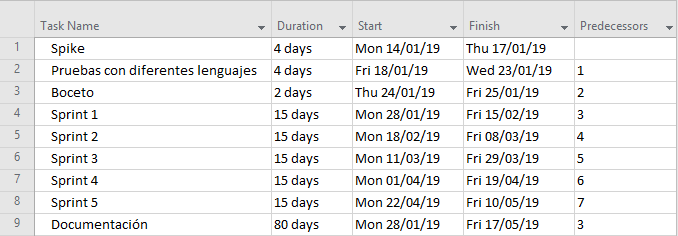
\includegraphics[scale=0.7]{planificacion-inicial-tareas.png}}
            \caption{Planificación de las fases del proyecto}
            \label{fig:gantt-initial-tasks}
        \end{figure}
        
        \begin{figure}[H]
        \centering
            \frame{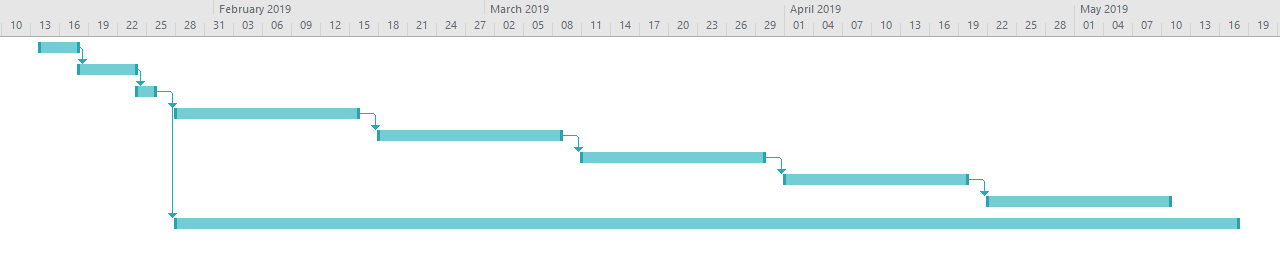
\includegraphics[scale=0.44]{planificacion-inicial-diagrama.png}}
            \caption{Diagrama de \textit{Gantt} de la planificación inicial}
            \label{fig:gantt-initial-diagram}
        \end{figure}
        
    \subsection{Seguimiento del proyecto}
        
        Las figuras \ref{fig:gantt-followup-tasks} y \ref{fig:gantt-followup-diagram} muestran la planificación detallada de las tareas del proyecto. Es importante destacar que debido a actividades no relacionadas con la aplicación, o actividades que aunque sean relacionadas con la aplicación no son incluidas en este proyecto, el proceso de desarrollo se ha visto afectado en ciertos momentos, reflejándose estas afectaciones como retrasos.
        
        \begin{figure}[H]
        \centering
            \frame{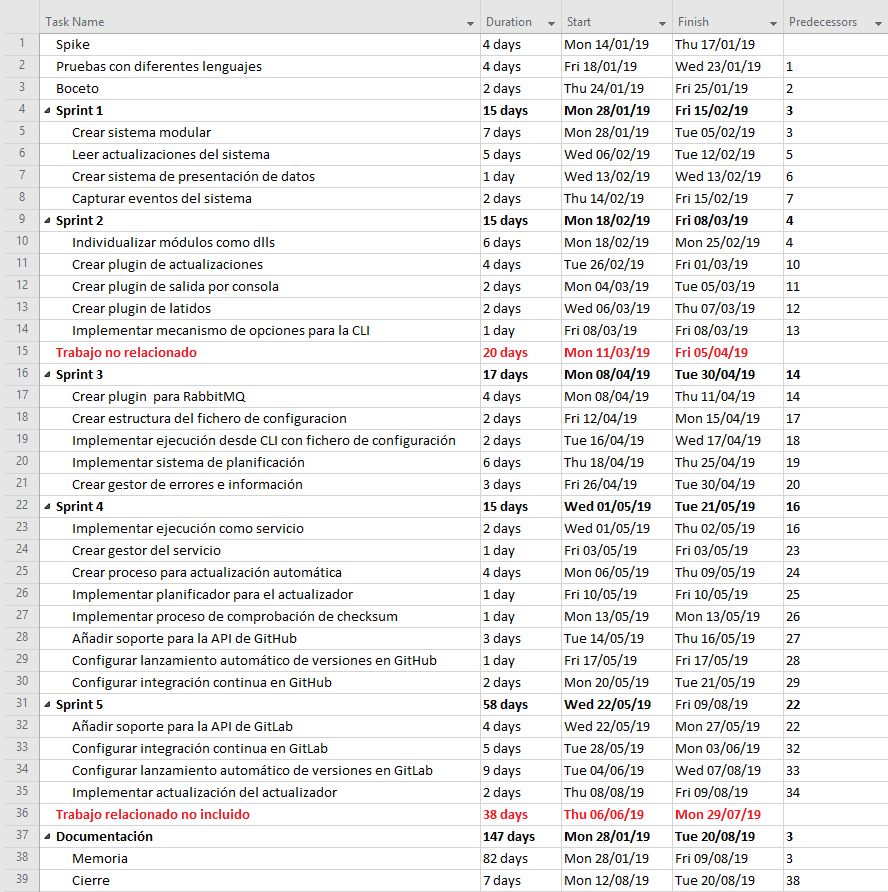
\includegraphics[scale=0.6]{seguimiento-tareas.png}}
            \caption{Planificación de las tareas del proyecto}
            \label{fig:gantt-followup-tasks}
        \end{figure}
    
        \begin{figure}[H]
        \centering
            \frame{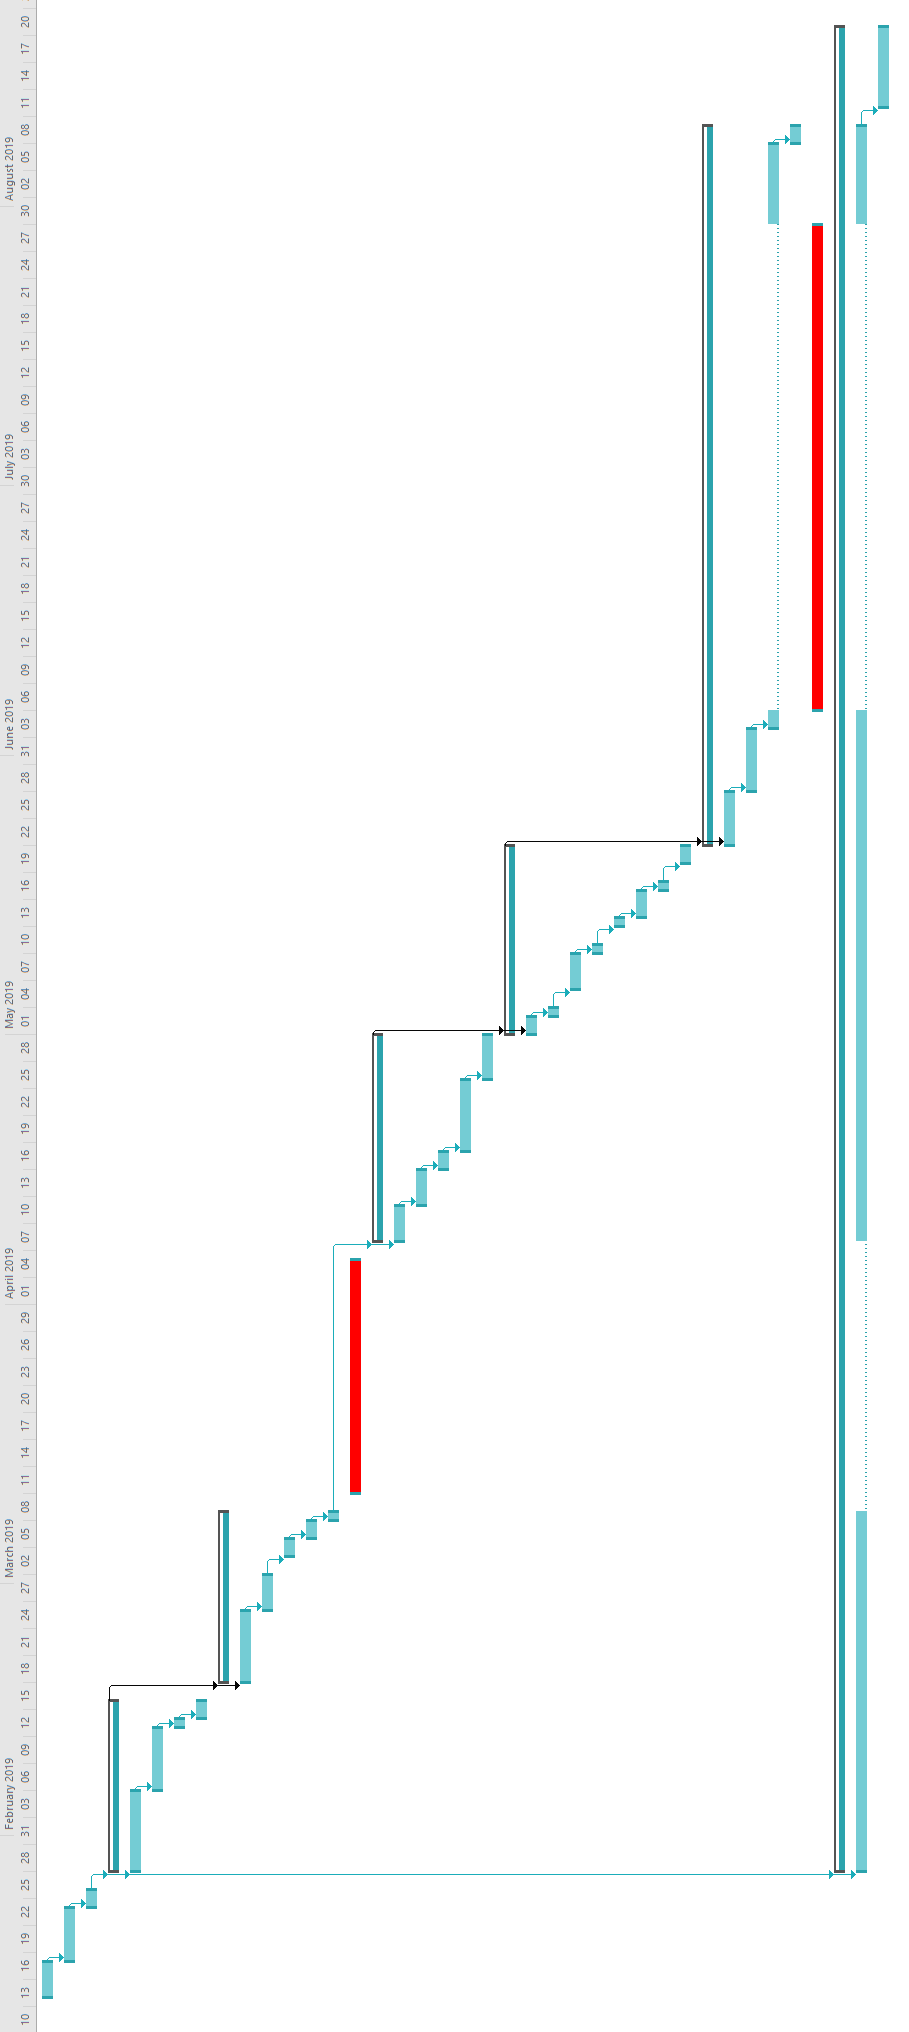
\includegraphics[scale=0.44]{seguimiento-diagrama.png}}
            \caption{Diagrama de \textit{Gantt} de la planificación de tareas}
            \label{fig:gantt-followup-diagram}
        \end{figure}